% =============================================================================
\section{GHZM states}
% =============================================================================

We also perform mesoscopic Schr\"odinger cat state simulations, corresponding to recent ion-trap experiments with $M$ qubits.
These states violate a genuine multipartite Bell inequality, which means that it is impossible to confine the Bell violation to a microscopic part of the state.
Such inequalities require the measurement of all possible correlation functions at the highest order available.
We find two distinct scaling laws for the total computational difficulty, as measured by the number of samples required to obtain a given sampling error.

To understand the ultimate scaling properties of probabilistic sampling methods, we have also simulated higher order correlations that violate multipartite Bell inequalities.
These are found in quantum states that display Bell violations with $M$ observers, not just two.
The most well-known examples are the multimode entangled Greenberger-Horne-Zeilinger-Mermin (\abbrev{ghzm}) states~\cite{Greenberger1989,Mermin1990}, corresponding to ``Schr\"odinger Cat'' states.
We therefore considered \abbrev{ghzm} states which describe $M$ spin-$\frac{1}{2}$ particles or qubits:
\begin{eqn}
    \vert\Phi\rangle
    = \frac{1}{\sqrt{2}} \left(
        \ket{\uparrow\ldots\uparrow}
        + e^{i\phi} \ket{\downarrow\ldots\downarrow}
    \right).
\end{eqn}
Here $\ket{\uparrow}$ and $\ket{\downarrow}$ denote spin-up or spin down particles in the $z$-direction.
As well as being of deep significance in quantum physics, such mesoscopic states have been generated in recent ion-trap experiments~\cite{Rowe2001,Leibfried2005,Monz2011}.
Quantum paradoxes are obtained on measuring an operator $\hat{A}$ which is defined as a linear combination of $2^{M}$ distinct $M$-th order correlation functions:
\begin{eqn}
    \hat{A}
    = \prod_{j=1}^{M} \left(
        \hat{\sigma}_{x}^{j}
        + i s_{j} \hat{\sigma}_{y}^{j}
        \right) e^{-i s_{j} \theta_{j}}.
\end{eqn}
For odd $M$ we follow Mermin~\cite{Mermin1990} and take $\phi=-\pi/2$, $s_{j}=1$ and $\theta_{j}=0$.
For even $M$ we follow Ardehali~\cite{Ardehali1992} and take $\phi=\pi$, $s_{j}=-1$ and $\theta_{j}=0$ for $j<M$, and $s_{M}=1$, $\theta_{M}=-\pi/4$.
Genuine multipartite Bell violations are known to exist for these states, which imply that the observed correlations cannot be explained by a nonlocality shared among $M-1$ or fewer qubits.
To test for genuine multipartite Bell nonlocality, we adopt the hybrid local-nonlocal \abbrev{lhv} model introduced by Svetlichny~\cite{Svetlichny1987} and Collins \textit{et al}~\cite{Collins2002}.



\begin{figure}
    \centerline{%
    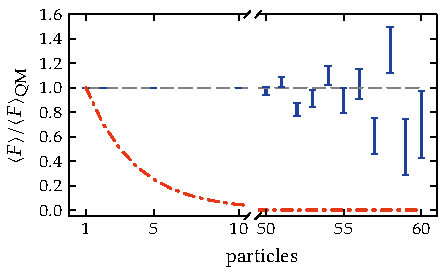
\includegraphics{figures_generated/bell/ghz_violations.pdf}%
    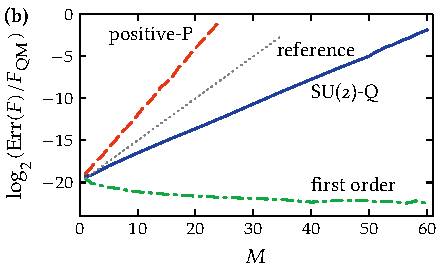
\includegraphics{figures_generated/bell/ghz_errors.pdf}}

    \caption{
    Violations for multi-particle \abbrev{ghz} states.
    (a) Simulated Mermin violation using SU(2)-Q representation.
    The values of expectations and errors are normalized by the quantum mechanical prediction for the corresponding $M$.
    The horizontal grey dashed line gives the quantum prediction.
    The error bars show the sampled result and estimated sampling errors at each value of $M$.
    The red dash-dotted line is the LHV prediction, which gives a Bell violation when above this line.
    Genuine multipartite Bell violations occur for $F_{\mathrm{sample}}/F_{\mathrm{QM}}>1/\sqrt{2}$.
    (b) Relative errors for F (blue line) and first order correlation, or total number of ``spin-ups'' (green dashed line) using SU(2)-Q representation.
    The dotted reference line shows the point at which the sampling errors would give scaling properties as slow as an experimental measurement.}

    \label{fig:bell-ineq:ghz:violation}
\end{figure}


\begin{figure}
    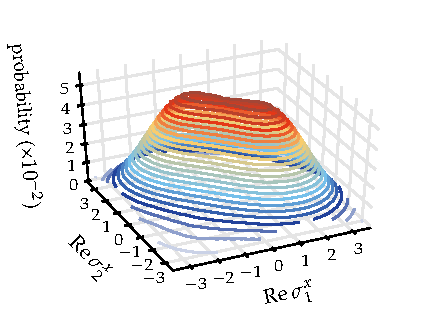
\includegraphics{figures_generated/bell/distribution_P1.pdf}%
    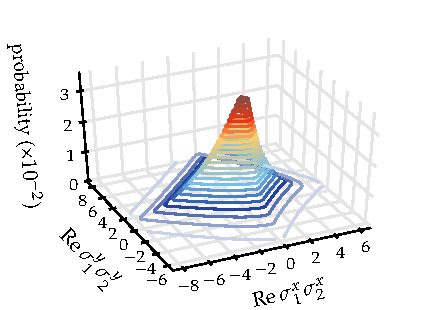
\includegraphics{figures_generated/bell/distribution_P2.pdf}\\
    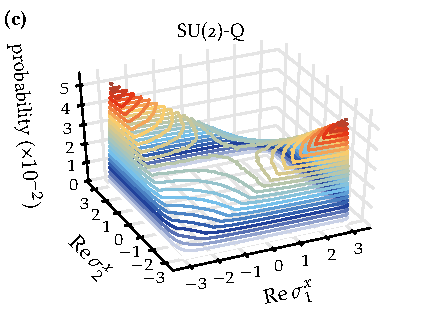
\includegraphics{figures_generated/bell/distribution_Q1.pdf}%
    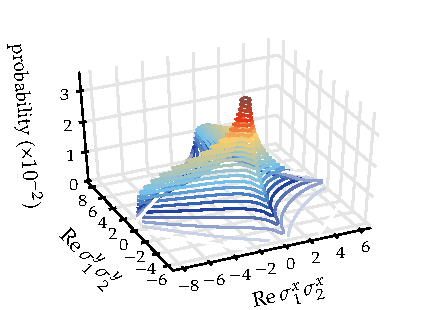
\includegraphics{figures_generated/bell/distribution_Q2.pdf}

    \caption{
    Correlations for the different parts of the quantity $F$, in case of positive-P (a, b) and SU(2)-Q (c, d) representations, $10^{8}$ samples.}

    \label{fig:bell-ineq:ghz:correlations}
\end{figure}

